\subsection{Accuracy of the model}
\label{sec:res-acc}

Figure~\ref{fig:accuracy} compares the predicted and measured iteration times of all \nAccN{} streaming configurations of the main runs (clocks locked, both model shapes, prefill and decode). The prediction uses the per-layer compute times scaled so that their sum equals the measured all-resident iteration (scale factors between \nCalScaleMin{} and \nCalScaleMax), and the per-layer copy times; nothing is fitted to the streaming runs. The mean absolute error is \nAccMape\% and the largest error \nAccMax\%. Without the scaling the mean error is \nAccMapeUncal\%. For the Llama-3.1-8B layer shapes the mean error is \nEightBMape\% (maximum \nEightBMax\%). The largest errors occur in decode iterations with most layers resident, where an iteration lasts less than about 120~ms and the host takes almost as long to enqueue the work; the model contains no host overhead. Over the \nAccRankPairs{} pairs of placements with the same workload, resident count and slots whose measured times differ by more than 2\%, the model orders \nAccRankPct\% correctly.

\begin{figure}[t]
\centering
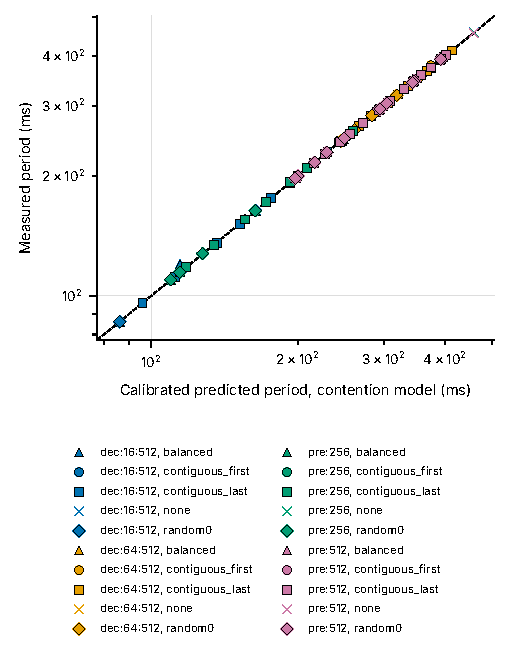
\includegraphics[width=0.75\linewidth]{figs/fig_accuracy.pdf}
\caption{Predicted versus measured iteration time for all streaming configurations of the main runs (Tesla T4, locked clocks). The line is $y=x$.}
\label{fig:accuracy}
\end{figure}

\subsection{Placement}
\label{sec:res-placement}

Figure~\ref{fig:penalty} shows, for each prefill length, the iteration time of the contiguous and balanced placements relative to the lower bound $\max(\sum c_i,\sum_{\text{streamed}} f_i)$ as the number of resident layers grows. The three regimes of Section~\ref{sec:theory} are visible. In the transfer-bound workloads ($T\le\nTransferBoundMaxT$, $f/c$ between \nRatioTransferMin{} and \nRatioTransferMax) the balanced placement stays at the bound for every $r$, while the contiguous one leaves the bound as soon as resident computation exceeds what $k$ slots can prefetch, and the gap widens until the resident layers' computation matches the streamed layers' copies. The largest measured gap is \nMeasPenaltyMax$\times$ (prefill of 256 tokens, $r=\nMeasPenaltyMaxR$, $k=\nMeasPenaltyMaxK$), and Theorem~\ref{thm:contig} predicts \nPredPenaltyAtMax$\times$. Contiguous-last behaves like contiguous-first, as the theory expects for any single block. Random placements fall in between; one random set of 21 layers that happened to contain a long resident run was \nRandomWorstPct\% slower than balanced. When a layer computes longer than it copies ($T\ge\nComputeBoundMinT$), all placements are within \nComputeBoundSpreadPct\% of each other and of the all-resident time, as Theorem~\ref{thm:compute} states. In decode the copies dominate unless almost all layers are resident, and placement matters only in the few configurations in which $rc$ approaches $mf$.

\begin{figure}[t]
\centering
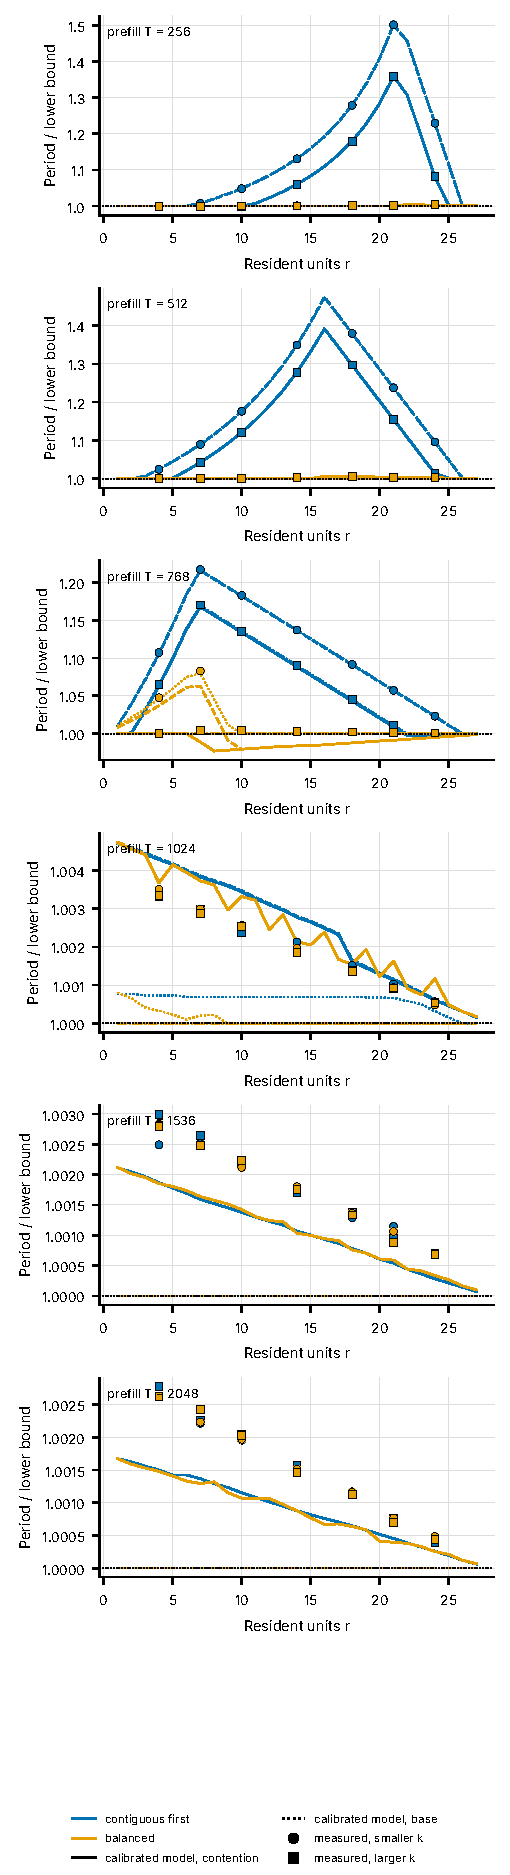
\includegraphics[width=\linewidth]{figs/fig_penalty.pdf}
\caption{Iteration time relative to the lower bound versus the number of resident layers, for contiguous-first and balanced placements (markers: measured; lines: model).}
\label{fig:penalty}
\end{figure}

Figure~\ref{fig:timeline} shows why. In the contiguous configuration the copy engine fills the slots while the resident block computes and then waits for most of the block; afterwards the streamed layers run at the copy rate. In the balanced configuration the copy engine is never idle and the iteration ends when the last copy has been consumed.

\begin{figure}[t]
\centering
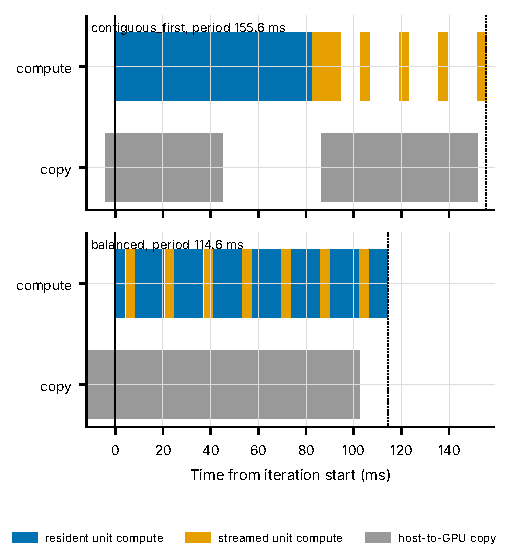
\includegraphics[width=\linewidth]{figs/fig_timeline.pdf}
\caption{Measured timelines of one iteration (prefill of 256 tokens, $r=21$, $k=3$) for contiguous-first (top) and balanced (bottom) placement. Each panel shows computation (upper row) and copies (lower row).}
\label{fig:timeline}
\end{figure}

\subsection{Number of slots}
\label{sec:res-slots}

At $T=768$ a layer copies in \nSweepRatio{} times its compute time, inside the band $c<f<2c$ of Proposition~\ref{prop:two}. Figure~\ref{fig:slots} shows the slot sweep for $r=14$. One slot serialises copy and computation. With two slots the balanced placement is \nSweepTwoOverThreePct\% slower than with three, as the proposition allows, and more slots do not help, as Theorem~\ref{thm:balanced} predicts. The model reproduces the sweep with a mean error of \nSweepMape\%.

\begin{figure}[t]
\centering
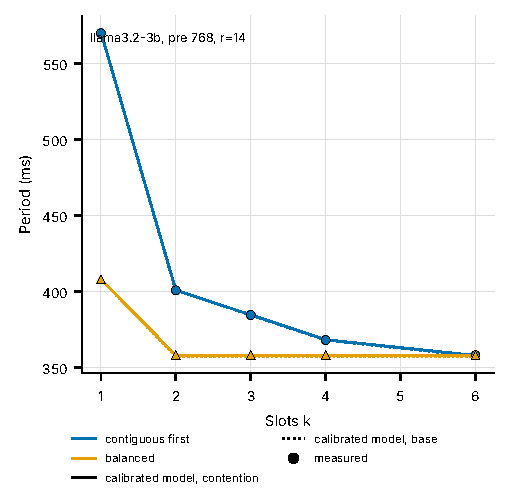
\includegraphics[width=0.75\linewidth]{figs/fig_slots.pdf}
\caption{Iteration time versus the number of slots at $T=768$, $r=14$ (markers: measured; lines: model).}
\label{fig:slots}
\end{figure}

\subsection{Non-uniform units: the output head}
\label{sec:res-nonuniform}

With the Llama-3.2 output head as an extra unit (788~MB, four times a layer, but computed for one token only), the model predicts the measured iterations with a mean error of \nHeadMape\%. Figure~\ref{fig:nonuniform} uses the measured per-unit times to compare placements under a memory budget. Streaming the head forces every slot to the head's size, so keeping the head resident and spreading the layers over the rest of the budget is \nNonUnifHeadGainPct\% faster than the balanced layer placement with a streamed head at the median budget; the local search finds placements within \nNonUnifLocalGainPct\% of this rule.

\begin{figure}[t]
\centering
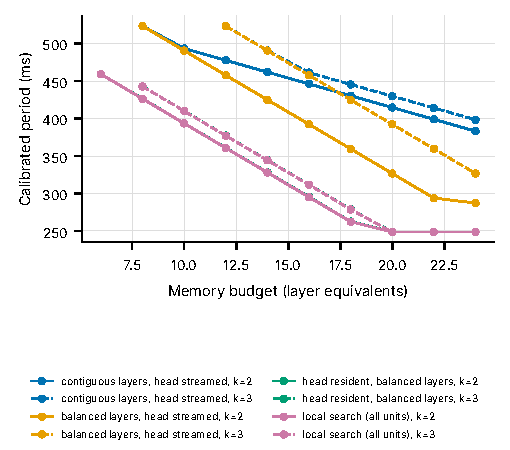
\includegraphics[width=0.75\linewidth]{figs/fig_nonuniform.pdf}
\caption{Predicted iteration time versus memory budget with the output head as a unit (prefill of 512 tokens): contiguous layers, balanced layers, head resident plus balanced layers, and local search.}
\label{fig:nonuniform}
\end{figure}

\subsection{Without clock locking}
\label{sec:res-power}

In runs whose SM clock fell below the locked value because of the power cap, the model with compute times from a cooler phase errs by up to \nCapMax\% (mean \nCapMape\%). Scaling each configuration's compute times by the ratio of the clock during the compute measurement to the clock during the run removes almost all of it (mean \nCapClockMape\%, maximum \nCapClockMax\%), so the error is the clock, not the pipeline model. In our first, fully unlocked runs the effect changed a conclusion: for a 1\,024-token prefill with 14 resident layers the balanced placement measured 374~ms against 364~ms for the contiguous one, although the model predicts the opposite. These runs had no clock samples, so we can only point to the mechanism shown above: with a balanced placement copies overlap computation for the whole iteration, which raises power draw and lowers the clock exactly while the computation is on the critical path.
